\chapter{Sudoku}
\label{sudoku}
\index{Sudoku}
\lettrine[nindent=0.1em]{S}{udoku} has become very popular recently as a puzzle. This logic puzzle involves working out the missing pieces in a $9\times{}9$ array of numbers: each row, column and quadrant must end up with the digits 1 to 9 with no repeats or omissions. Figure~\ref{su:unsolved} shows a typical presentation of a Sudoku puzzle, in its unsolved state of course.

\begin{figure}[h]
%\begin{boxed}
\centering
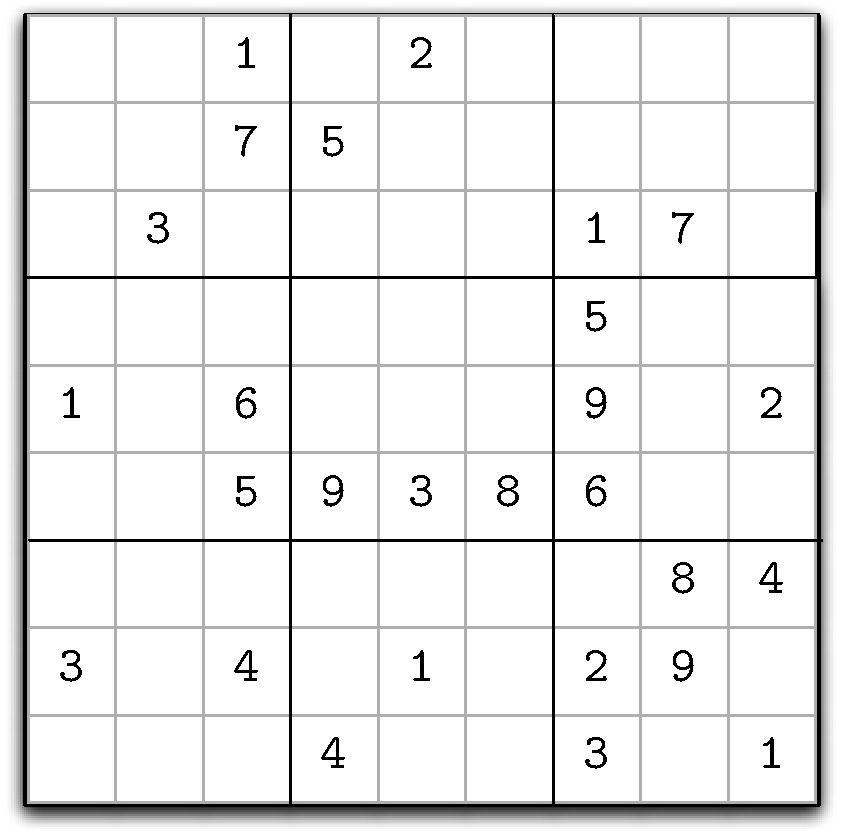
\includegraphics[width=2.5in]{unsolved}
%\end{boxed}
\caption{\label{su:unsolved}A typical sudoku puzzle}
\end{figure}

\noindent
The sudoku puzzle is an excellent opportunity to explore the capabilities of \go in problem solving and, in particular in constraint solving. As we shall see, our solution highlights a large number of \go's features; including the use of anonymous classes to achieve the effect of \q{let} in functional programming languages.

\section{Sudoku Strategy}
\label{su:strategy}
\index{Sudoku!strategy}

The key operation in solving a sudoku puzzle is the elimination of alternatives. We can represent the contents of a square as a set of alternative numbers to place there. At each step in the solution we will use the existing information to eliminate choices; until eventually, there are no choices in any of the squares and the puzzle is solved.

For example, the $6^{th}$ row in Figure~\vref{su:unsolved} has four blank spaces. Taking only the row itself into consideration, we can say that each of the blank squares can take on any of the numbers 1,2,4, or 7. That is because the other digits are already taken in that row. However, for a given cell, we must not only take into account the other cells in the same row, but we must also take into account the other cells in the same column and the other cells in the same $3\times{}3$ quadrant that the cell is in.

Taking these into account, the $6^{th}$ row can be represented as in Figure~\ref{su:sixth}.

\begin{figure}[h]
%\begin{boxed}
\centering
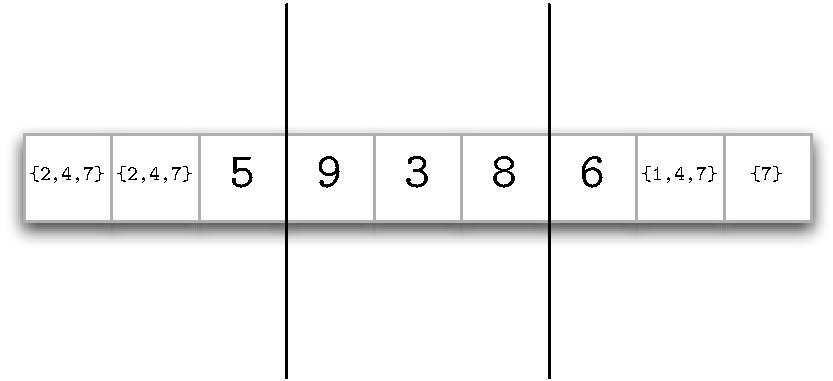
\includegraphics[width=2.5in]{sixth}
%\end{boxed}
\caption{\label{su:sixth}An annotated row}
\end{figure}

\subsection{Selecting a single solution}
Notice that the last square in the row has just one element in its set of possibilities -- namely 7. That means that we can infer that that cell has the number 7 in it.

Based on that choice, in the next step we can assign 7 to the last cell and eliminate 7 from the other cells -- giving the situation as in Figure~\vref{su:seven}.

\begin{figure}[h]
%\begin{boxed}
\centering
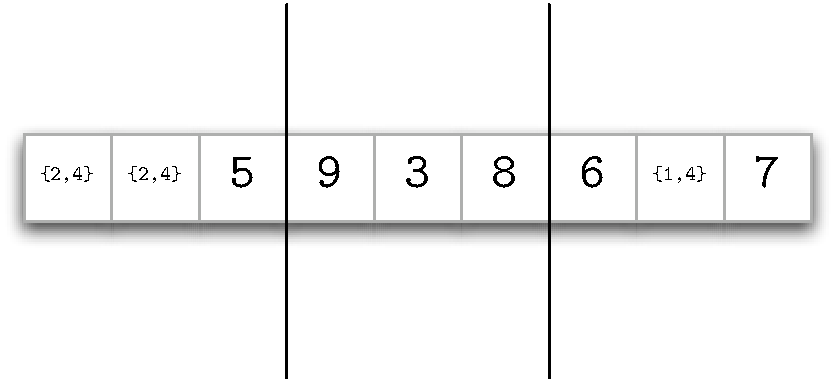
\includegraphics[width=2.5in]{seven}
%\end{boxed}
\caption{\label{su:seven}After selecting 7}
\end{figure}

\subsection{Unique elements}
In Figure~\vref{su:seven} we have reduced the possibilities to 2 or 4 in the first two cells and one of 1,2 or 4 in the $8^{th}$ cell. Notice that although this $8^{th}$ cell has three possibilities, it is the only cell in the row that the number $1$ appears in.

That means that we can infer that the $8^{th}$ cell must contain the number $1$ in it: even though currently there are three possibilities for that cell; the fact that we must be able to place all the digits and this is the only choice for $1$ allows us to assign $1$ to the $8^{th}$ cell. We show the resulting situation in Figure~\vref{su:one}.

\begin{figure}[h]
%\begin{boxed}
\centering
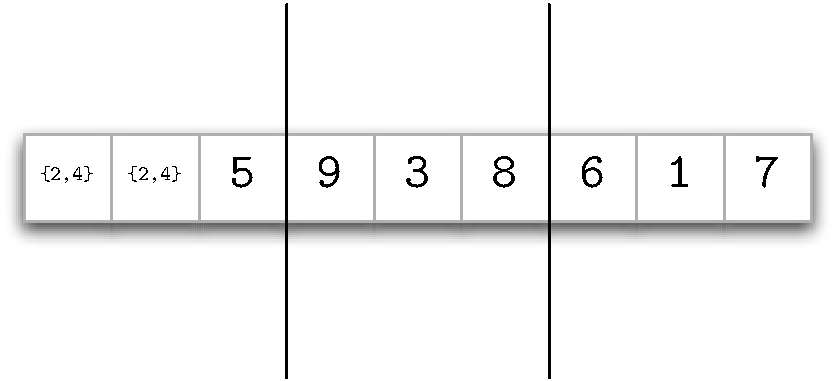
\includegraphics[width=2.5in]{one}
%\end{boxed}
\caption{\label{su:one}After assigning 1 to the $8^{th}$ cell}
\end{figure}
\noindent
After these steps we are left with both of the first two cells having the choice set \q{\{2,4\}}; and without further information we cannot infer any further constraints. However, solving the puzzle will involve iteratively looking at every row, column and quadrant in the same way.

\subsection{Cycling}
\label{su:cycle}
Thus a reasonable strategy for solving sudoku puzzles is the repeated application of three rules:
\begin{enumerate}
\item
Eliminate from cells' possible solutions any digit that has already be assigned to any cell in the same row, column or quadrant;
\item
If a cell's set of possibilities is reduced to one, then assign that number to the cell; and
\item
If a cell's set of possibilities contains a number that is not present in any of the other cells' possible sets in a given row, column or quadrant; then assign that number to the cell.
\end{enumerate}
\begin{aside}
It should never happen that a given cell's possible assignments contains \emph{more than one} choice which is not in any of the other cells' choices. That would be an unsolvable sudoku puzzle.

Again, if the set of choices for a cell is empty, then that puzzle also has no solution.
\end{aside}
Our program will solve sudoku puzzles by iteratively applying these rules to each row, column and quadrant until no further progress is possible.

By tradition, sudoku puzzles are deterministically solveable. However, a particularly fiendish puzzle setter may choose to \emph{under determine} the puzzle. In this case a puzzle solver is left with a set of constraints that cannot be further tightened by applying these rules and to solve the puzzle choices must be made.

Our program will steadfastly refuse to solve such puzzles and simply leave the puzzle in the partially solved state. It would, however, be relatively straight forward to extend the program to non-deterministically choose a partial solution and continue with the regular solving. If the solution attempt fails then a different choice would have to be made; until either solution is found or no solution is possible.

\section{Representing a sudoku puzzle}
The groundwork for our sudoku puzzler solver is the set of structures that we can use to represent the current state of the solver's problem. We do this with two key concepts: the structures needed to represent the choices in an individual cell in the square and the square as a collection of cells.

\subsection{Representing choices}
\label{su:choice}

At the heart of our sudoku solver is the notion of a set of possible choices for a given cell. Solving the puzzle involves progressive manipulation of this set of choices until only one choice remains -- the digit that must be assigned to that cell.

We can represent a set of choices as a \q{list[]} of \q{integer}s. However, we need to be able to manipulate this set, and so we shall \emph{encapsulate} the state of a cell in a stateful \q{constr} object.\note{A slightly more natural terminology would have been \q{cell}; however, that risks confusion with the standard \q{cell} package.}

We start our program by defining the type interface that defines the actions that we can perform on the set of choices of a cell:
\begin{alltt}
constr \impl \{
  curr:[]\funarrow{}list[integer].
  remove:[integer]*. assign:[integer]*.
\}.
\end{alltt}
There are three things that we can do with a cell's choices: find out what the \q{curr}ent set of choices is, we can \q{remove} a digit from the set, and we can \q{assign} a number to the cell.

It will also be convenient if we can have a consistent way of showing the contents of a cell's choices. However, since, all types inherit from the standard \q{thing} type, we do not need to explicitly call out the \q{show} type in the interface for \q{constr}.

Program~\vref{su:constr} shows an implementation of this type (sans any explicit \q{show} function. The current set of possible solutions is held in an object variable -- \q{L}; and this list represents the basis for reporting the \q{curr}ent set, q{remov}ing elements and so on.
\begin{program}
\vspace{0.5ex}
\begin{alltt}
constr:[list[integer]]\sconarrow{}constr.
constr(L0)..\{
  L:list[integer] := L0.

  curr()=>L.

  remove(K) ->
    L := L \bsl{} [K].

  assign(K) ->
    ( K in L ? 
      L := [K]).
\}.
\end{alltt}
\vspace{-2ex}
\caption{Recording choices in a cell}
\label{su:constr}
\end{program}
The \q{remove} program uses an operator that we have not yet encountered in our exploration of \go: the \q{\bsl{}} set subtraction operator. This, together with other set operations is defined in a standard \go package: \q{go.setlib}. The \q{\bsl{}} operator is special in that it is a standard operator of the \go language, but its implementation is strictly conventional:\note{This is an illustrative implementation of the set subtraction operator.}
\begin{alltt}
L\bsl{}M => \{ e .. (e::\nasf{}e in M) in L \}
\end{alltt}

The \q{go.setlib} package offers a set-like layer on top of ordinary \go lists -- by providing operators that preserve the setness property. I.e., if \q{L} and \q{M} are set-like lists (with no duplicate entries), then the result of subtracting \q{M} from \q{L} will also be set-like. The other set operators supported by \q{go.setlib} are set union (\q{\union}) and set intersection (\q{\intersection}).

Program~\ref{su:constr}'s function is really to \emph{record} the result of applying constraints to the cell -- the constraints arising from sudoku itself do not appear here.

\subsection{A Sudoku Square}
\label{su:table}
\index{Suduko!representing the square}

The kinds of rules that we discussed in Section~\vref{su:cycle} imply that we need to process the complete sudoku square in a number of different ways: processing each row of the square, each column of the square and each quadrant of the square. Traditionally, laying out a matrix like this seems to imply a choice: whether to have the matrix in row-column form or in column-row form. A row-column layout favors column-oriented processing, and a column-row layout favors row-oriented processing. However, because we also need to be able to process the table both in row-orientation and in column orientation. Furthermore, we \emph{also} need to support quadrant-oriented processing. This will strongly affect how we represent the cells in the sudoku square.

Manipulating a square array in this way is not especially unique to Sudoku (although it is not all that often that one needs to process the quadrants of a matrix). In particular, we do \emph{not} need to tie it to the contents of each cell: we are accessing rows, columns, etc., but they could be row of anything. I.e. this suggests a polymorphic type interface to the \q{square} concept:
\begin{alltt}
square[t] \typearrow{} \{ 
  colOf:[integer]\funarrow{}list[t]. 
  rowOf:[integer]\funarrow{}list[t].
  quadOf:[integer]\funarrow{}list[t].
  cellOf:[integer,integer]\funarrow{}t.
  row:[integer]\{\}.
  col:[integer]\{\}.
  quad:[integer]\{\}.
\}.
\end{alltt}
For example, we shall use the \q{colOf} function to extract a column from the table -- as a vector represented as a list. Similarly the \q{quadOf} function will also return a particular vector from the table -- corresponding to the particular quadrant.

The \q{row}, \q{col} and \q{quad} predicates are defined over ranges of \q{integer}s which indicate the indices of the legal rows, columns and quadrants in the table. Note that we do not \emph{bake} into this interface the size of the square. In fact, we can have any size square that we want.
\begin{aside}
The size of a sudoku square has to be itself a perfect square. We can have a $4\times{}4$ sudoku square, a $16\times{}16$ sudoku square and so on; but a $5\times{}5$ square does not have quadrants that also have 5 elements in them.
\end{aside}
Program~\vref{su:square} shows the outer aspects of a class that implements the \q{square} interface.
\begin{program}
\vspace{0.5ex}
\begin{alltt}
square:[list[t]]\sconarrow{}square[t].
square(Init)..\{
  Els:list[t] = Init.
  Sz:integer = itrunc(sqrt(listlen(Init))).

  row(I) :- I in iota(1,Sz).
  col(I) :- I in iota(1,Sz).
  quad(I) :- I in iota(1,Sz).
  \ldots{}
\}.
\end{alltt}
\vspace{-2ex}
\caption{Top-level of a \q{square} class}
\label{su:square}
\end{program}
The \q{square} class constructor (it is a stateful constructor) takes as its argument a list of entries -- which is assumed to take the form of a linear list of all the entries in the square in row-order. The class has -- at this stage -- two internal object variables: the list of \q{Els} and the length of the square. For a $9\times{}9$ square, the list of entries should contain 81 elements and the variable \q{Sz} will be computed as $9$ from that list.

Note that since we cannot decide whether the square will be processed in primarily row-order or column-order (or quadrant order) we do not attempt to \emph{structure} the entries in any way: we simply leave it as a linear list. We will will do is access this list in ways that are consistent with the row-ordering or column-ordering. However, the elements of the list are effectively in row-ordering; as in Figure~\vref{su:elements}.
\begin{figure}[h]
%\begin{boxed}
\centering
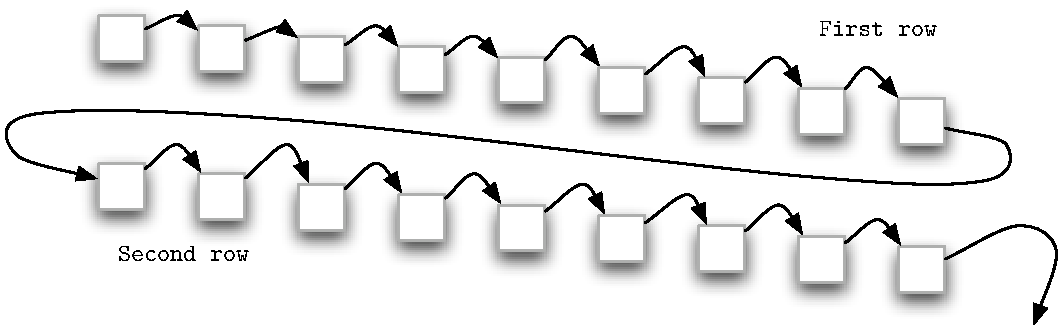
\includegraphics[width=3in]{elements}
%\end{boxed}
\caption{\label{su:elements}The elements in a \q{square} list}
\end{figure}
\noindent
It is arguable that a linear list is not an efficient way of representing the elements of a matrix. However, it is a simple technique and for our purposes efficient enough.

\subsubsection{Accessing a \q{row} out of the \q{square}}
The \q{square} interface allows us to extract the \emph{$n^{th}$} row as a separate list of elements. Since the list of elements is in row order, to access a given row we simply have to select the appropriate contiguous selection from the list of elements. To do this we use two functions that are part of \go's standard list-processing library: \q{drop} and \q{front}. 

The \q{front} function returns the first \emph{n} elements of a list, and \q{drop} is the converse: it returns the remaining elements after the $n^{th}$ element.
Program~\vref{su:rowof} shows how we can achieve this simply -- note that we are assuming that the first row, column and quadrant in the \q{square} is numbered from 1. The \q{rowOf} function is assumed to be textually within the class body for \q{square}.
\begin{program}
\vspace{0.5ex}
\begin{alltt}
rowOf(i) => front(drop(Els,(i-1)*Sz),Sz).
\end{alltt}
\vspace{-2ex}
\caption{Accessing a \q{rowOf} the square}
\label{su:rowof}
\end{program}

\subsubsection{Accessing a \q{col}umn out of the \q{square}}
Given that the list of elements in the \q{square} is in row order, accessing a column is slightly more complex: we have to access a cell from each row. 

The first cell in the column is at a position that depends on the number of the column. However, thereafter, successive elements of the column will always be a fixed distance away in the list -- the size of square governs this distance.

Program~\vref{su:colof}, which also should be viewed as being embedded in the \q{square} class body, shows how we can extract the elements that correspond to the column. We use an auxiliary function to access the subsequent elements from the list of \q{Els}. Note that \q{clOf} drops \q{Sz-1} elements from the list because that is the number of elements \emph{between} each element of a given column.
\begin{program}
\vspace{0.5ex}
\begin{alltt}
colOf(i) => clOf(drop(Els,(i-1)*Sz)).
  
clOf:[list[t]]=>list[t].
clOf([])=>[].
clOf([El,..L]) => [El,..clOf(drop(L,Sz-1))].
\end{alltt}
\vspace{-2ex}
\caption{Accessing a \q{colOf} the square}
\label{su:colof}
\end{program}
\noindent
The \q{clOf} recursion ends with the empty list; this works because \q{drop} will return an empty list if asked to drop more elements than are in the list. (This will be true after the last element of the column has been extracted.)

\subsubsection{Accessing a quadrant of the square}
Quadrants are a little like a combination of a row and a column: each row in the quadrant is contiguous within the list of elements, and successive rows in the quadrant are separated by a fixed number of other elements. Figure~\vref{su:quadrant} shows how the third quadrant is formed out of segments from the list.
\begin{figure}[h]
%\begin{boxed}
\centering
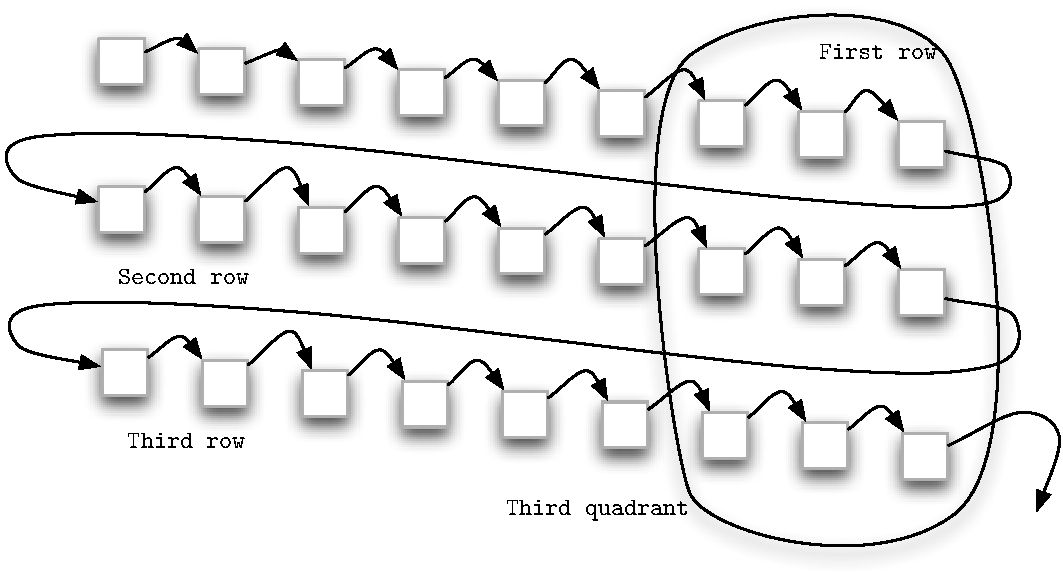
\includegraphics[width=3in]{quadrant}
%\end{boxed}
\caption{\label{su:quadrant}The elements in a quadrant}
\end{figure}
\noindent
Thus, once we have located the first row associated with the quadrant within the list of elements, extracting the rows of the quadrant is straightforward. We have to be a little more careful than when extracting the elements of a column as we will generally not be processing every row; and the gap between quadrant rows is less than the gap between entire rows.

Program~\vref{su:quad-1} shows how the successive elements of a quadrant are extracted.
\begin{program}
\vspace{0.5ex}
\begin{alltt}
Sq:integer = itrunc(sqrt(Sz)).

qdOf:[list[t],integer] => list[t].
qdOf(_,0)=>[].
qdOf(L,Cnt) => front(L,Sq)<>qdOf(drop(L,Sz),Cnt-1).
\end{alltt}
\vspace{-2ex}
\caption{Accessing the rows of a quadrant}
\label{su:quad-1}
\end{program}
\noindent
The \q{qdOf} function has two arguments: the list of elements to process and the number of segments to extract. The \q{Sq} object constant gives the length of each quadrant row (it is the square root of the length \q{Sz} of the square itself).

The tricksiest aspect of extracting a quadrant is deciding where to start extracting elements. If the size of the square is \q{Sz}, each row has $\sqrt{Sz}$ quadrants laid across it (a $9\times9$ square has three quadrants in each row, a $16\times16$ square will have 16 quadrants in total overlaying in a $4\times4$ grid over the square).

Similarly, there are $\sqrt{Sz}$ rows in a given quadrant. The total number of cells in a 'row of quadrants' is $\sqrt{Sz}\times{}Sz$ cells. For example, in a $9\times9$ square, each row of quadrants is 27 cells.

Thus the $i^{th}$ quadrant originates at cell
\[
((i-1)//\sqrt{Sz})\times\sqrt{Sz}\times{}Sz+(i-1)|\sqrt{Sz}
\]
where $A//B$ means the integer part of the quotient of $A/B$ and $A|B$ means the modulus of $A$ with respect to $B$. The computation with the integer quotient and modulus is required to select the quadrant's row of in the rows of quadrants.

For example, in a $16\times16$ square, the fifth quadrant (recall that that will be the first quadrant in the second row of quadrants) will be at cell 
\[
((5-1)//\sqrt{16})\times\sqrt{16}\times16+(5-1)|\sqrt{16} = 64
\]
We use this calculation in Program~\vref{su:quad-2} to initiate the extraction of the segments of the appropriate quadrant.
\begin{program}
\vspace{0.5ex}
\begin{alltt}
Sz2:integer = Sq*Sq*Sq.   -- compute Sz^1.5

\ldots{}
quadOf(i) => qdOf(drop(Els,
                     ((i-1) quot Sq)*S2+imod((i-1),Sq)*Sq),
                  Sq).
\end{alltt}
\vspace{-2ex}
\caption{Finding the right quadrant}
\label{su:quad-2}
\end{program}

\begin{aside}
After this, we leave the computation needed to access a single cell of the square to the reader!
\end{aside}

\section{Solving the Sudoku puzzle}
\label{su:solve}
\index{Sudoku!solving the puzzle}

The key to our algorithm is the repeated application of the rules that we identified in Section~\vref{su:cycle}. These are essentially the application of two kinds of filter, and the subsequent assignment of answers.

\subsection{Constraint filters}
\label{su:filter}

There are two kinds of filters that we need to apply: the elimination of impossible numbers from the sets of choices, and the identification of unique choices -- leading to the selection and subsequent elimination of the selection from other cells.

\subsubsection{Elimination filter}
The elimination filter has the very simple task of removing a specific number from the choices available to a given row, column or quadrant. Given the form of the \q{square} interface, we will be able to apply each filter in a uniform manner: to a list of choices represented as \q{constr} objects.

Program~\vref{su:elim} shows the elimination filter: it is given a list of \q{constr} objects and a number to eliminate; and it eliminates it. The only issue is to make sure that if a \q{constr} contains \emph{only} the number to elimnate then we \emph{do not} eliminate it from that \q{constr}. The reason is that we use such structures to represent the situation where a number has been assigned to the cell.
\begin{program}
\vspace{0.5ex}
\begin{alltt}
elim:[list[constr],integer]*.
elim(Set,K) ->
  (El in Set *>
    (K in El.curr(), El.curr()\bsl=[K]?
      \{\}
    | El.remove(K); done:=false
    )
  ).
\end{alltt}
\vspace{-2ex}
\caption{Elimination filter}
\label{su:elim}
\end{program}
\noindent
We perform one additional chore in the \q{elim} action procedure: we set a global variable \q{done} to \q{false} whenever we actually \q{remove} an element from a set of choices. We will use this later to govern the overall cycling of the sudoku solver. This is also the reason for the slightly long-winded test:
\begin{alltt}
K in El.curr(), El.curr()\bsl=[K]
\end{alltt}
We only want to set the \q{done} variable when we are actually progressing the solving of the puzzle.

We can use \q{elim} from Program~\vref{su:elim} to write the elimination filter for a complete set. Program~\vref{su:singleton} searches a set for a singleton element and, if it finds one, uses that to apply the \q{elim} filter to the other elements of the set.
\begin{program}
\vspace{0.5ex}
\begin{alltt}
singleton:[list[constr]]*.
singleton(Set) ->
  ( El in Set *>
    ( El.curr()=[K] ?  -- do we have a singleton?
      elim(Set,K)
    | \{\}
    )
  )
\end{alltt}
\vspace{-2ex}
\caption{Filtering for singletons}
\label{su:singleton}
\end{program}

\subsubsection{Uniqueness filter}
The complement case for singleton elements is where a given choice contains a number that does not appear in any other choice. In that case we can assign the cell that choice -- and subsequently the singleton filter will remove that choice from the other elements of the set.

Finding a unique element of a set of choices means finding an element that does not occur elsewhere. The \q{unique} predicate defined in Program~\vref{su:unique} is satisfied of a digit \q{U} if there is a nontrivial element in the set of choices that has \q{U} in it, and that \q{U} does not appear elsewhere in the set.
\begin{program}
\vspace{0.5ex}
\begin{alltt}
unique:[list[constr],constr,integer]\{\}.
unique(Set,Ot,U) :-
  append(F,[Ot,..B],Set),
  Cn = Ot.curr(), nontrivial(Cn),
  U in Cn, 
  \nasf(E in F, U in E.curr()),
  \nasf(E in B, U in E.curr()). 
\end{alltt}
\vspace{-2ex}
\caption{Finding unique choices}
\label{su:unique}
\end{program}
Program~\vref{su:unique} is formulated slightly differently to the \q{singleton} filter in Program~\vref{su:singleton}: we are using a call to the standard predicate \q{append} to non-deterministically \emph{partition} the set into three  pieces: a front piece (we call \q{F}), a back piece (we call \q{B}) and the element in the middle. The query
\begin{alltt}
append(F,[El,..B],Set)
\end{alltt}
accomplishes all of that. 

The two query conditions of the form
\begin{alltt}
\nasf(E in F, U in E.curr())
\end{alltt}
and
\begin{alltt}
\nasf(E in B, U in E.curr())
\end{alltt}
verify that the selected \q{U} does not appear in the \q{F} and \q{B} pieces.

Note that if there is no suitable candidate then the \q{unique} filter will \emph{fail}; a fact that we make use of in Program~\vref{su:uniqueset} which applies the \q{unique} filter where possible.
\begin{program}
\vspace{0.5ex}
\begin{alltt}
findUnique:[list[constr]]*.
findUnique(Set) ->
  ( unique(Set,Ot,U) *>
	 Ot.assign(U); done:=false
  ).
\end{alltt}
\vspace{-2ex}
\caption{Filtering for unique choices}
\label{su:uniqueset}
\end{program}
Note that, here also, we set the global \q{done} variable to \q{false} when we actually make a change to the choices in the set.

\subsection{A filter cycle}
The filters that we established in Section~\vref{su:filter} need to be applied to each row, column and quadrant in the square. This will involve iterating over those rows, columns and quadrants. This, in turn, builds on the \q{rowOf}, \q{colOf} and \q{quadOf} functions that we defined in Section~\vref{su:table}.

Program~\vref{su:applyall} shows one straightforward way of tackling this iteration: we define an auxiliary procedure \q{filterSet} that applies all the filters to a given row, column or quadrant. A complete cycle involves applying \q{filterSet} to each possible row, column and quadrant.
\begin{program}
\vspace{0.5ex}
\begin{alltt}
filterSet:[list[constr]]*.
filterSet(Set) ->
	singleton(Set);
	findUnique(Set).

applyAll:[square[constr]]*
applyAll(Square) ->
  ( Square.rowOf(R) *> filterSet(R));
  ( Square.colOf(R) *> filterSet(R));
  ( Square.quadrantOf(R) *> filterSet(R)).
\end{alltt}
\vspace{-2ex}
\caption{Apply filters}
\label{su:applyall}
\end{program}

\subsubsection{Are we done yet?}
Our strategy for solving a sudoku puzzle is inherently iterative. When a filter reduces the set of choices, or makes a selection, we rely on that action resulting in the potential for more constraints to be applied. In this way, constraints \emph{propagate} throughout the problem space until no more constraints trigger.

Only when no constraint can be applied can we ask whether we have solved the puzzle or not: if, when no further filters apply, there are only singleton sets in the square, then we know that we have solved the puzzle.

Recall that in the filter programs we set a global variable whenever we actually applied one of the filters. We will now use this global variable to control the cycles. In fact, \q{done} is not a truly global variable, we will put it -- together with the filter programs -- inside an \emph{anonymous} class; used as a kind of \q{let} expression.

\go does not directly have the kind of \q{let} expression that one encounters in functional programming languages. However, it is not needed either. First of all, let us define a somewhat simple type interface that will allow us to \q{do} things:
\begin{alltt}
do \impl \{ do:[]* \}
\end{alltt}
If we had a class that implemented this type, it may look like:
\begin{alltt}
do:[]\sconarrow{}do.
do..\{
  done:logical := false.
  
  do()::done -> \{\}.
  do() ->
    done := true;
    \ldots     -- possibly reset done
    do().
\}
\end{alltt}
This form is a pattern that can be used to govern a certain kind of iteration where the condition that governs the loop is not easily centralized (as in our case).

We have seen a number of examples of \go classes where the definition is essentially statically defined at the top-level of the package. However, \go supports classes in other contexts as well: classes can be defined \emph{inside} other classes -- i.e., inner classes (see Section~\vref{lo:inner}). In fact, classes can be defined \emph{in-line}: an \emph{anonymous} class
\index{anonymous class}
is simultaneously a class definition, and an occurrence of its constructor. We can use this to achieve the equivalent of \q{let} expressions. Program~\vref{su:cycleall} shows how we create an anonymous instance of the \q{do} type, and invoke its \q{do} action method to iterate our puzzle solver.

\begin{program}
\vspace{0.5ex}
\begin{alltt}
  solve:[square[constr]]*.
  solve(S) ->
    (:do..\{
      done:logical:=false.
      
      do()::done -> \{\}.
      do() ->
        done:=true;
        applyAll(S);
        do().
        
      \ldots
      applyAll:[square[constr]]*
      \ldots
    \}).do().
\end{alltt}
\vspace{-2ex}
\caption{Solving the sudoku}
\label{su:cycleall}
\end{program}
The construction:
\begin{alltt}
:do..\{ \ldots \}
\end{alltt}
is the anonymous class being defined. Like all programs, it must be declared and the type of this anonymous class is \q{do}. 

An anonymous class is called anonymous because there is no real name for the class; because it is simultaneously a class definition and a constructor for the class, the only handle is the object value of the anonymous class expression.

Our \q{solve} action procedure in Program~\vref{su:cycleall} creates the anonymous instance and invokes its \q{do} action method.

Note that the variable \q{S} is not passed explicitly into \q{do} -- it is a \emph{free variable} of the anonymous class. \go arranges that the correct value is supplied to the \q{applyAll} action call. Similarly, the \q{done} variable is free in the various filter programs -- all of which must be textually located within the \q{do} anonymous class otherwise the variable \q{done} will not be accessible to them.

\subsection{Putting it all together}
We have now established all the major pieces of our sudoku solver. Our final task is to arrange for the solver to be given the puzzle to solve, and to display the solution. 

In a complete application we would construct the puzzle to solve by reading a description of the puzzle from the keyboard. However, for the sake of brevity we will not be doing that in this chapter. 

The complete \q{sudoku} solver, including some details omitted here, is shown in Section~\vref{sample:sudoku}

